\frame
{

\begin{center}
 \Huge{Inteligencia de Negocios en PostgreSQL}
\end{center}

\vfill

\begin{columns}

\begin{column}{0.3\textwidth}
\end{column}
\begin{column}{0.7\textwidth}
\raggedleft \footnotesize
The research leading to these results has received funding from the European Union's \href{http://ec.europa.eu/research/fp7/index_en.cfm}{\underline{Seventh Framework Programme (FP7/2007-2013)}} under grant agreement n° 318633
\end{column}
\end{columns}
}

\frame
{ \frametitle{¿Qué es “inteligencia de negocios”?}

{\Large “Inteligencia de negocios”}: traducción del término
\emph{Business Intelligence} (BI)

\vfill

{\raggedleft
”habilidades, tecnologías, aplicaciones y prácticas
que se utilizan para ayudar a una organización a
adquirir una mejor comprensión de su contexto comercial”}

\vfill

\pause
{\small En otras palabras:}
\vfill
\raggedleft{
\alert{Utilización de datos sobre el pasado y el presente
para tomar mejores decisiones en el futuro.}}

}

\frame
{ \frametitle{Inteligencia de negocios: Objetivos}

	\large{Requisito}
	\begin{itemize}
		\item Tenemos los datos
		\item (idealmente muchos de ellos)
	\end{itemize}

	\vfill \pause

	\large{Objetivos:}
	\begin{itemize}
		\item Queremos explorar estos datos ...
		\item ... y descubrir el conocimiento escondido en ellos
	\end{itemize}
}
% 
% \frame
% { \frametitle{Inteligencia de negocios: Tecnologías}
% 
% Normalmente BI incluye tecnologías como:
% 
% \begin{itemize}
% 	\item Data Warehousing
% 	\item On-Line Analytical Processing
% 	\item Data mining
% \end{itemize}
% 
% }

%\frame
%{ \frametitle{Inteligencia de negocios: Arquitecturas: Dos capas}
%	\includegraphics[width=0.6\paperwidth]{two-layer-architecture.png}
%}

\frame
{ \frametitle{Inteligencia de negocios: Arquitectura de tres capas}

	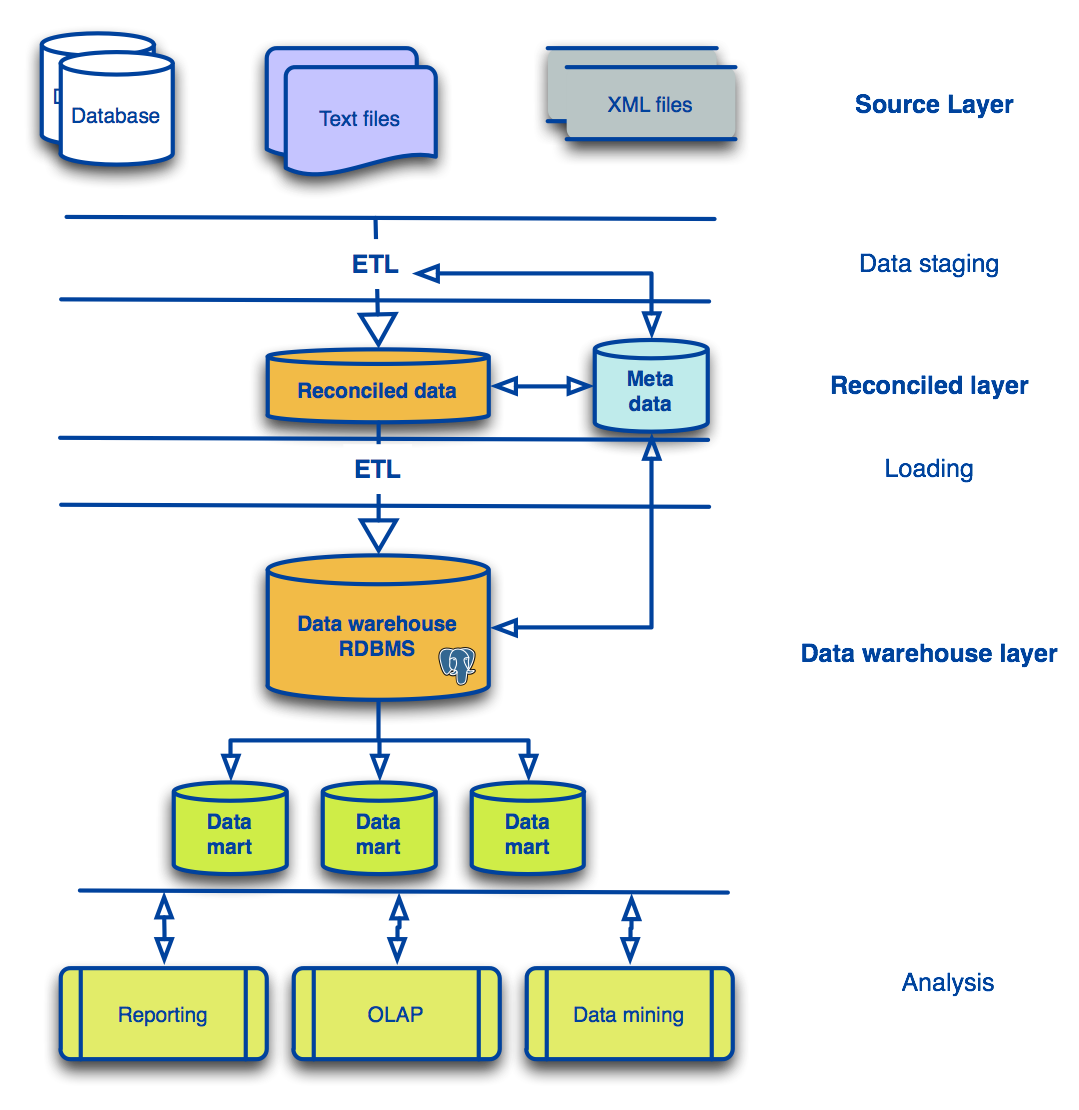
\includegraphics[width=0.6\paperwidth]{three-layer-architecture.png}

	\note[enumerate]{
Capa origen: múltiples fuentes de datos operacionales, múltiples fuentes de datos externas (archivos planos, documentos, XML, web services)

Cuarentena de datos: los datos de la capa fuente son extraidos y transformados (limpiados, validados, integrados) y finalmente cargados. A este proceso se le llama ETL

Metadatos: se usan para definir procesos aplicar a los datos fuente (transformaciones, agregaciones, localizaciones, etc).  Puede no existir.

Data mart: subconjunto o agregación de un data warehouse; para mejorar rendimiento.
}
}

% \frame
% { \frametitle{Inteligencia de negocios: Arquitecturas: Bus}
%	\includegraphics[width=0.6\paperwidth]{bus-architecture.png}
% }
% 
% \frame
% { \frametitle{Inteligencia de negocios: Arquitecturas: DWH federado}
%	\includegraphics[width=0.6\paperwidth]{federated-architecture.png}
% }


\frame
{ \frametitle{¿En qué ayuda Postgres?}
	{\Large En esta arquitectura de tres capas:}

	\vfill
	\begin{enumerate}
		\item	Cuarentena y carga de datos (\emph{stage and load})
		\item	Almacenes de datos (\emph{data warehouse}, \emph{data marts})
		\item	Ejecución de consultas (\emph{analysis})
	\end{enumerate}
}

\section{Cuarentena y Carga de datos}
\frame{
		\huge{Cuarentena y Carga de datos}
}

\frame
{ \frametitle{Herramientas ETL}

\begin{itemize}
	\item \emph{\Large Extract -- Transform -- Load}
	\item Cargar datos externos en variedad de formatos
	\item Lidiar con errores e inconsistencias
	\item Manipular los datos antes de insertarlos
	\item PGLoader: \url{http://www.pgloader.io}
\end{itemize}
}

\frame
{ \frametitle{Aproximación ELT}

\begin{itemize}
	\item \emph{\Large Extract -- Load -- Transform}
	\item El proceso de transformación se hace dentro de la BD
	\item La transformación puede usar herramientas de PostgreSQL
\end{itemize}
}

\frame
{ \frametitle{Conectores de datos externos}

\begin{itemize}
	\item \emph{Foreign Data Wrappers (FDW)}
	\item Conectar, desde Postgres, a servidores de datos remotos
	\item (En realidad, a cualquier cosa que provea datos)
	\item El mecanismo es extensible: puedes escribir el tuyo
	\item \url{http://wiki.postgresql.org/wiki/FDW}

\item \tiny
 postgres\_fdw
 oracle\_fdw
 mysql\_fdw
 odbc\_fdw
 jdbc\_fdw
 informix\_fdw
 firebird\_fdw
 sqlite\_fdw
 tds\_fdw
 couchdb\_fdw
 MonetDB FDW
 mongo\_fdw
 redis\_fdw
 Neo4j fdw
 Tycoon FDW
 file\_fdw
 file\_text\_array\_fdw
 file\_fixed\_length\_record\_fdw
 json\_fdw
 twitter\_fdw
 ldap\_fdw
 PGStrom
 Hadoop FDW
 s3\_fdw
 www\_fdw
 cstore\_fdw
 {\bf multicorn }


\end{itemize}
}

\section{Almacenes de datos}
\frame{
	\huge{Almacenes de Datos}
}

\frame[containsverbatim]
{ \frametitle{Soporte extensivo JSON}

\begin{itemize}
	\item Tipos de datos \texttt{JSON} (9.2) y \texttt{JSONB} (9.4)
	\item Almacenamiento semi-estructurado
	\item Facilita el acceso a datos de proveniencia no relacional
	\item Indexable (índices GIN, GiST)
\end{itemize}

\begin{verbatim}
  { "id" : "142857",
    "nombre" : "Javier González",
    "nacimiento" : { "fecha" : "1976/10/14",
                     "lugar" : { "pais" : "Venezuela" }
                   },
  }
\end{verbatim}

}

\frame[containsverbatim]
{ \frametitle{Vistas Materializadas}
\begin{itemize}
	\item \emph{Materialized views}
	\item Útil para data-mart
		\begin{itemize}
			\item tiene otros usos también
		\end{itemize}
	\item Permite generar “resúmenes” de datos que pueden ser consultados repetidamente
	\item Mejora el rendimiento en consultas repetitivas sobre los mismos resúmenes
	\item Simplifica refresco de vistas resúmenes según necesidades de la organización
\end{itemize}

\pause

\begin{verbatim}
CREATE MATERIALIZED VIEW vm AS
   SELECT u, d, t
     FROM tab_1 JOIN tab_2 ...
    WHERE ...

REFRESH MATERIALIZED VIEW vm;
\end{verbatim}
}

\frame
{ \frametitle{Tables “unlogged”}

\begin{itemize}
	\item \emph{UNLOGGED TABLES}
	\item Tablas que no son respaldadas en WAL
	\item Mejora en rendimiento de escrituras por ahorrar tráfico WAL
	\item Desventaja es perder datos en caso de caída
	\pause
	\item En un \emph{DWH} o \emph{data mart} no importa
		\begin{itemize}
			\item los datos pueden volver a crearse
			\item es un riesgo aceptable porque las caídas son infrecuentes
				\begin{itemize}
					\item o deberían serlo
				\end{itemize}
		\end{itemize}
\end{itemize}
}

\frame
{ \frametitle{Hot Standby}

\begin{itemize}
	\item Permite tener una copia de datos en un servidor separado
	\item ... el cual puede ejecutar consultas de sólo lectura
	\item Para ejecutar reportes
		\begin{itemize}
			\item sin sobrecargar el servidor en operación OLTP
		\end{itemize}
	\item Puede tener réplicas “en cascada”
		\begin{itemize}
			\item distribuir geográficamente
			\item \emph{high availability}
			\item tomar respaldos \emph{pg\_dump}
		\end{itemize}
\end{itemize}
}

\frame
{ \frametitle{En desarrollo: UDR}

\begin{itemize}
	\item \emph{Uni-Directional Replication} (replicación uni-direccional)
	\item Replicación a nivel lógico, no físico
		\begin{itemize}
			\item como Slony, Londiste
		\end{itemize}
	\item Permite hacer cambios en la réplica
		\begin{itemize}
			\item a diferencia de \emph{hot standby}
			\item tablas temporales
			\item índices adicionales
		\end{itemize}
	\item Proyecto en desarrollo de 2ndQuadrant
	\item Basado en BDR: \url{http://wiki.postgresql.org/wiki/BDR}
\end{itemize}
}

\section{Ejecución de consultas}
\frame{
	\huge{Ejecución de Consultas}
}

\frame
{ \frametitle{Funciones y Procedimientos en la base}
\begin{itemize}
	\item Muchos procesos se pueden ejecutar en la base
	\item Ahorra tráfico de datos
	\item Programas definidos por el usuario ...
		\begin{itemize}
			\item implementar lógica de negocio
		\end{itemize}
	\item ... en una variedad de lenguajes
	\item Mantener el conocimiento en la base
		\begin{itemize}
			\item Permite reutilizar en múltiples herramientas
		\end{itemize}
\end{itemize}
}


\frame
{ \frametitle{MADlib}
\begin{itemize}
	\item \url{http://madlib.net}
	\item \emph{MADlib: Big Data Machine Learning in SQL for Data Scientists}
	\item Powerful analytics for Big Data
	\item También \texttt{PL/R}
		\begin{itemize}
			\item análisis estadístico, etc
			\item visualizaciones de datos (gráficos, etc)
		\end{itemize}
\end{itemize}
}

\logo{\href{http://www.2ndquadrant.com/}{
\includegraphics[height=1cm]{axle-logo-weights.jpg}}}
\frame[containsverbatim]
{ \frametitle{En desarrollo: Aggregate pushdown}

\begin{itemize}
	\item Ejecuta la agregación más cerca del recorrido de la tabla
	\item Permite ahorrar movimiento de datos a través de nodos de ejecución que no lo necesitan
\end{itemize}

\tiny
\begin{verbatim}
WITH w_ventas AS ( 
SELECT ventas_valor_pagado, ventas_cliente_id
FROM ventas, dim_fechas
WHERE fechas_anno = 2001
        AND fechas_fecha = ventas_fecha
        AND ventas_cliente IS NOT NULL
), w_clientes AS (
SELECT clientes_cliente_id
FROM clientes, clientes_detalles
WHERE clientes_cliente_id = detalles_cliente_id
        AND detalle_estado_credito = 'Bueno'
        AND detalle_genero = 'F'
)
SELECT clientes_cliente_id, sum(ventas_valor_pagado) as total_pagado
FROM w_ventas, w_clientes
WHERE
    ventas_cliente_id = clientes_cliente_id
GROUP BY clientes_cliente_id
HAVING total_pagado > 0
ORDER BY total_pagado DESC
LIMIT 100;
\end{verbatim}

%\pause
%
%\begin{verbatim}
%  SELECT uno, dos, max(precio)
%    FROM (SELECT ... , precio
%            FROM ventas
%	   WHERE ...)
%GROUP BY ..
%\end{verbatim}
}


\logo{\href{http://www.2ndquadrant.com/}{
\includegraphics[height=1cm]{2ndQuadrant_150.jpg}}}

\frame
{ \frametitle{Bitmap index scan}

\begin{itemize}
	\item Recorrer un índice, generar un bitmap
	\item El bitmap permite recorrer la tabla en orden físico
	\item El bitmap puede ser operado con otro bitmap
		\begin{itemize}
			\item  de otro o del mismo índice
		\end{itemize}
\end{itemize}
\pause
\begin{center}
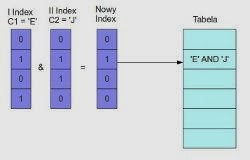
\includegraphics[width=0.5\textwidth]{Bitmap_scan2.jpg}
\end{center}
}

\frame[containsverbatim]
{ \frametitle{Funciones de ventana deslizante}

\begin{itemize}
	\item Permiten escribir consultas complejas
	\item Análisis de conjuntos de datos
\end{itemize}

\begin{verbatim}
SELECT departamento, empleado_id, salario,
       avg(salario) OVER (PARTITION BY departamento) AS a,
       rank() OVER (PARTITION BY departamento
                    ORDER BY salario DESC) AS r
FROM salario_empleados
ORDER BY r
\end{verbatim}
\pause

\begin{itemize}
	\item Ahorran mucho código en la aplicación
	\item (bugs, lentitud, HH desarrollo)
\end{itemize}
}

\logo{\href{http://www.2ndquadrant.com/}{
\includegraphics[height=1cm]{axle-logo-weights.jpg}}}
\frame
{ \frametitle{En desarrollo: BRIN indexes}
\begin{itemize}
	\item (Anteriormente llamados \emph{Minmax indexes})
	\item Índices para acelerar recorridos secuenciales
	\item Guardar valores min() y max() de la columna, para grupos de páginas
\end{itemize}
}

\frame {

% Graphic for TeX using PGF
% Title: /home/alvherre/brin.dia
% Creator: Dia v0.97.3
% CreationDate: Wed Oct 22 09:51:03 2014
% For: alvherre
% \usepackage{tikz}
% The following commands are not supported in PSTricks at present
% We define them conditionally, so when they are implemented,
% this pgf file will use them.
\ifx\du\undefined
  \newlength{\du}
\fi
\setlength{\du}{15\unitlength}
\begin{tikzpicture}
\pgftransformxscale{1.000000}
\pgftransformyscale{-1.000000}
\definecolor{dialinecolor}{rgb}{0.000000, 0.000000, 0.000000}
\pgfsetstrokecolor{dialinecolor}
\definecolor{dialinecolor}{rgb}{1.000000, 1.000000, 1.000000}
\pgfsetfillcolor{dialinecolor}
\definecolor{dialinecolor}{rgb}{1.000000, 1.000000, 1.000000}
\pgfsetfillcolor{dialinecolor}
\fill (3.972347\du,3.603643\du)--(3.972347\du,5.503643\du)--(6.072347\du,5.503643\du)--(6.072347\du,3.603643\du)--cycle;
\pgfsetlinewidth{0.100000\du}
\pgfsetdash{}{0pt}
\pgfsetdash{}{0pt}
\pgfsetmiterjoin
\definecolor{dialinecolor}{rgb}{0.000000, 0.000000, 0.000000}
\pgfsetstrokecolor{dialinecolor}
\draw (3.972347\du,3.603643\du)--(3.972347\du,5.503643\du)--(6.072347\du,5.503643\du)--(6.072347\du,3.603643\du)--cycle;
% setfont left to latex
\definecolor{dialinecolor}{rgb}{0.000000, 0.000000, 0.000000}
\pgfsetstrokecolor{dialinecolor}
\node at (5.022347\du,4.748643\du){3};
\definecolor{dialinecolor}{rgb}{1.000000, 1.000000, 1.000000}
\pgfsetfillcolor{dialinecolor}
\fill (6.059847\du,3.603643\du)--(6.059847\du,5.503643\du)--(8.059847\du,5.503643\du)--(8.059847\du,3.603643\du)--cycle;
\pgfsetlinewidth{0.100000\du}
\pgfsetdash{}{0pt}
\pgfsetdash{}{0pt}
\pgfsetmiterjoin
\definecolor{dialinecolor}{rgb}{0.000000, 0.000000, 0.000000}
\pgfsetstrokecolor{dialinecolor}
\draw (6.059847\du,3.603643\du)--(6.059847\du,5.503643\du)--(8.059847\du,5.503643\du)--(8.059847\du,3.603643\du)--cycle;
% setfont left to latex
\definecolor{dialinecolor}{rgb}{0.000000, 0.000000, 0.000000}
\pgfsetstrokecolor{dialinecolor}
\node at (7.059847\du,4.748643\du){10};
\definecolor{dialinecolor}{rgb}{1.000000, 1.000000, 1.000000}
\pgfsetfillcolor{dialinecolor}
\fill (8.047347\du,3.603643\du)--(8.047347\du,5.503643\du)--(9.865522\du,5.503643\du)--(9.865522\du,3.603643\du)--cycle;
\pgfsetlinewidth{0.100000\du}
\pgfsetdash{}{0pt}
\pgfsetdash{}{0pt}
\pgfsetmiterjoin
\definecolor{dialinecolor}{rgb}{0.000000, 0.000000, 0.000000}
\pgfsetstrokecolor{dialinecolor}
\draw (8.047347\du,3.603643\du)--(8.047347\du,5.503643\du)--(9.865522\du,5.503643\du)--(9.865522\du,3.603643\du)--cycle;
% setfont left to latex
\definecolor{dialinecolor}{rgb}{0.000000, 0.000000, 0.000000}
\pgfsetstrokecolor{dialinecolor}
\node at (8.956434\du,4.748643\du){1};
\definecolor{dialinecolor}{rgb}{1.000000, 1.000000, 1.000000}
\pgfsetfillcolor{dialinecolor}
\fill (3.972347\du,5.500000\du)--(3.972347\du,7.400000\du)--(6.294847\du,7.400000\du)--(6.294847\du,5.500000\du)--cycle;
\pgfsetlinewidth{0.100000\du}
\pgfsetdash{}{0pt}
\pgfsetdash{}{0pt}
\pgfsetmiterjoin
\definecolor{dialinecolor}{rgb}{0.000000, 0.000000, 0.000000}
\pgfsetstrokecolor{dialinecolor}
\draw (3.972347\du,5.500000\du)--(3.972347\du,7.400000\du)--(6.294847\du,7.400000\du)--(6.294847\du,5.500000\du)--cycle;
% setfont left to latex
\definecolor{dialinecolor}{rgb}{0.000000, 0.000000, 0.000000}
\pgfsetstrokecolor{dialinecolor}
\node at (5.133597\du,6.645000\du){100};
\definecolor{dialinecolor}{rgb}{1.000000, 1.000000, 1.000000}
\pgfsetfillcolor{dialinecolor}
\fill (6.059847\du,5.500000\du)--(6.059847\du,7.400000\du)--(8.047347\du,7.400000\du)--(8.047347\du,5.500000\du)--cycle;
\pgfsetlinewidth{0.100000\du}
\pgfsetdash{}{0pt}
\pgfsetdash{}{0pt}
\pgfsetmiterjoin
\definecolor{dialinecolor}{rgb}{0.000000, 0.000000, 0.000000}
\pgfsetstrokecolor{dialinecolor}
\draw (6.059847\du,5.500000\du)--(6.059847\du,7.400000\du)--(8.047347\du,7.400000\du)--(8.047347\du,5.500000\du)--cycle;
% setfont left to latex
\definecolor{dialinecolor}{rgb}{0.000000, 0.000000, 0.000000}
\pgfsetstrokecolor{dialinecolor}
\node at (7.053597\du,6.645000\du){20};
\definecolor{dialinecolor}{rgb}{1.000000, 1.000000, 1.000000}
\pgfsetfillcolor{dialinecolor}
\fill (8.047347\du,5.475000\du)--(8.047347\du,7.375000\du)--(9.867767\du,7.375000\du)--(9.867767\du,5.475000\du)--cycle;
\pgfsetlinewidth{0.100000\du}
\pgfsetdash{}{0pt}
\pgfsetdash{}{0pt}
\pgfsetmiterjoin
\definecolor{dialinecolor}{rgb}{0.000000, 0.000000, 0.000000}
\pgfsetstrokecolor{dialinecolor}
\draw (8.047347\du,5.475000\du)--(8.047347\du,7.375000\du)--(9.867767\du,7.375000\du)--(9.867767\du,5.475000\du)--cycle;
% setfont left to latex
\definecolor{dialinecolor}{rgb}{0.000000, 0.000000, 0.000000}
\pgfsetstrokecolor{dialinecolor}
\node at (8.957557\du,6.620000\du){-5};
% setfont left to latex
\definecolor{dialinecolor}{rgb}{0.000000, 0.000000, 0.000000}
\pgfsetstrokecolor{dialinecolor}
\node[anchor=west] at (6.931029\du,5.892511\du){};
\definecolor{dialinecolor}{rgb}{1.000000, 1.000000, 1.000000}
\pgfsetfillcolor{dialinecolor}
\fill (11.014013\du,4.533333\du)--(11.014013\du,6.433333\du)--(14.414013\du,6.433333\du)--(14.414013\du,4.533333\du)--cycle;
\pgfsetlinewidth{0.100000\du}
\pgfsetdash{}{0pt}
\pgfsetdash{}{0pt}
\pgfsetmiterjoin
\definecolor{dialinecolor}{rgb}{0.000000, 0.000000, 0.000000}
\pgfsetstrokecolor{dialinecolor}
\draw (11.014013\du,4.533333\du)--(11.014013\du,6.433333\du)--(14.414013\du,6.433333\du)--(14.414013\du,4.533333\du)--cycle;
% setfont left to latex
\definecolor{dialinecolor}{rgb}{0.000000, 0.000000, 0.000000}
\pgfsetstrokecolor{dialinecolor}
\node at (12.714013\du,5.678333\du){-5, 100};
\definecolor{dialinecolor}{rgb}{1.000000, 1.000000, 1.000000}
\pgfsetfillcolor{dialinecolor}
\fill (3.966060\du,7.398014\du)--(3.966060\du,9.347828\du)--(6.084847\du,9.347828\du)--(6.084847\du,7.398014\du)--cycle;
\pgfsetlinewidth{0.100000\du}
\pgfsetdash{}{0pt}
\pgfsetdash{}{0pt}
\pgfsetmiterjoin
\definecolor{dialinecolor}{rgb}{0.000000, 0.000000, 0.000000}
\pgfsetstrokecolor{dialinecolor}
\draw (3.966060\du,7.398014\du)--(3.966060\du,9.347828\du)--(6.084847\du,9.347828\du)--(6.084847\du,7.398014\du)--cycle;
% setfont left to latex
\definecolor{dialinecolor}{rgb}{0.000000, 0.000000, 0.000000}
\pgfsetstrokecolor{dialinecolor}
\node at (5.025453\du,8.567921\du){42};
\definecolor{dialinecolor}{rgb}{1.000000, 1.000000, 1.000000}
\pgfsetfillcolor{dialinecolor}
\fill (6.059847\du,7.398014\du)--(6.059847\du,9.322828\du)--(8.052025\du,9.322828\du)--(8.052025\du,7.398014\du)--cycle;
\pgfsetlinewidth{0.100000\du}
\pgfsetdash{}{0pt}
\pgfsetdash{}{0pt}
\pgfsetmiterjoin
\definecolor{dialinecolor}{rgb}{0.000000, 0.000000, 0.000000}
\pgfsetstrokecolor{dialinecolor}
\draw (6.059847\du,7.398014\du)--(6.059847\du,9.322828\du)--(8.052025\du,9.322828\du)--(8.052025\du,7.398014\du)--cycle;
% setfont left to latex
\definecolor{dialinecolor}{rgb}{0.000000, 0.000000, 0.000000}
\pgfsetstrokecolor{dialinecolor}
\node at (7.055936\du,8.555421\du){2};
\definecolor{dialinecolor}{rgb}{1.000000, 1.000000, 1.000000}
\pgfsetfillcolor{dialinecolor}
\fill (8.047347\du,7.373014\du)--(8.047347\du,9.322828\du)--(9.876513\du,9.322828\du)--(9.876513\du,7.373014\du)--cycle;
\pgfsetlinewidth{0.100000\du}
\pgfsetdash{}{0pt}
\pgfsetdash{}{0pt}
\pgfsetmiterjoin
\definecolor{dialinecolor}{rgb}{0.000000, 0.000000, 0.000000}
\pgfsetstrokecolor{dialinecolor}
\draw (8.047347\du,7.373014\du)--(8.047347\du,9.322828\du)--(9.876513\du,9.322828\du)--(9.876513\du,7.373014\du)--cycle;
% setfont left to latex
\definecolor{dialinecolor}{rgb}{0.000000, 0.000000, 0.000000}
\pgfsetstrokecolor{dialinecolor}
\node at (8.961930\du,8.542921\du){5};
\definecolor{dialinecolor}{rgb}{1.000000, 1.000000, 1.000000}
\pgfsetfillcolor{dialinecolor}
\fill (3.976076\du,9.319935\du)--(3.976076\du,11.219935\du)--(6.064013\du,11.219935\du)--(6.064013\du,9.319935\du)--cycle;
\pgfsetlinewidth{0.100000\du}
\pgfsetdash{}{0pt}
\pgfsetdash{}{0pt}
\pgfsetmiterjoin
\definecolor{dialinecolor}{rgb}{0.000000, 0.000000, 0.000000}
\pgfsetstrokecolor{dialinecolor}
\draw (3.976076\du,9.319935\du)--(3.976076\du,11.219935\du)--(6.064013\du,11.219935\du)--(6.064013\du,9.319935\du)--cycle;
% setfont left to latex
\definecolor{dialinecolor}{rgb}{0.000000, 0.000000, 0.000000}
\pgfsetstrokecolor{dialinecolor}
\node at (5.020045\du,10.464935\du){2};
\definecolor{dialinecolor}{rgb}{1.000000, 1.000000, 1.000000}
\pgfsetfillcolor{dialinecolor}
\fill (6.059847\du,9.319935\du)--(6.059847\du,11.219935\du)--(8.039013\du,11.219935\du)--(8.039013\du,9.319935\du)--cycle;
\pgfsetlinewidth{0.100000\du}
\pgfsetdash{}{0pt}
\pgfsetdash{}{0pt}
\pgfsetmiterjoin
\definecolor{dialinecolor}{rgb}{0.000000, 0.000000, 0.000000}
\pgfsetstrokecolor{dialinecolor}
\draw (6.059847\du,9.319935\du)--(6.059847\du,11.219935\du)--(8.039013\du,11.219935\du)--(8.039013\du,9.319935\du)--cycle;
% setfont left to latex
\definecolor{dialinecolor}{rgb}{0.000000, 0.000000, 0.000000}
\pgfsetstrokecolor{dialinecolor}
\node at (7.049430\du,10.464935\du){37};
\definecolor{dialinecolor}{rgb}{1.000000, 1.000000, 1.000000}
\pgfsetfillcolor{dialinecolor}
\fill (8.039497\du,9.319935\du)--(8.039497\du,11.219935\du)--(9.872347\du,11.219935\du)--(9.872347\du,9.319935\du)--cycle;
\pgfsetlinewidth{0.100000\du}
\pgfsetdash{}{0pt}
\pgfsetdash{}{0pt}
\pgfsetmiterjoin
\definecolor{dialinecolor}{rgb}{0.000000, 0.000000, 0.000000}
\pgfsetstrokecolor{dialinecolor}
\draw (8.039497\du,9.319935\du)--(8.039497\du,11.219935\du)--(9.872347\du,11.219935\du)--(9.872347\du,9.319935\du)--cycle;
% setfont left to latex
\definecolor{dialinecolor}{rgb}{0.000000, 0.000000, 0.000000}
\pgfsetstrokecolor{dialinecolor}
\node at (8.955922\du,10.464935\du){0};
% setfont left to latex
\definecolor{dialinecolor}{rgb}{0.000000, 0.000000, 0.000000}
\pgfsetstrokecolor{dialinecolor}
\node[anchor=west] at (6.907875\du,14.804430\du){};
\definecolor{dialinecolor}{rgb}{1.000000, 1.000000, 1.000000}
\pgfsetfillcolor{dialinecolor}
\fill (11.070122\du,8.418253\du)--(11.070122\du,10.318253\du)--(14.435122\du,10.318253\du)--(14.435122\du,8.418253\du)--cycle;
\pgfsetlinewidth{0.100000\du}
\pgfsetdash{}{0pt}
\pgfsetdash{}{0pt}
\pgfsetmiterjoin
\definecolor{dialinecolor}{rgb}{0.000000, 0.000000, 0.000000}
\pgfsetstrokecolor{dialinecolor}
\draw (11.070122\du,8.418253\du)--(11.070122\du,10.318253\du)--(14.435122\du,10.318253\du)--(14.435122\du,8.418253\du)--cycle;
% setfont left to latex
\definecolor{dialinecolor}{rgb}{0.000000, 0.000000, 0.000000}
\pgfsetstrokecolor{dialinecolor}
\node at (12.752622\du,9.563253\du){0, 42};
% setfont left to latex
\definecolor{dialinecolor}{rgb}{0.000000, 0.000000, 0.000000}
\pgfsetstrokecolor{dialinecolor}
\node[anchor=west] at (2\du,4.758333\du){pág1};
% setfont left to latex
\definecolor{dialinecolor}{rgb}{0.000000, 0.000000, 0.000000}
\pgfsetstrokecolor{dialinecolor}
\node[anchor=west] at (2\du,6.643661\du){pág2};
% setfont left to latex
\definecolor{dialinecolor}{rgb}{0.000000, 0.000000, 0.000000}
\pgfsetstrokecolor{dialinecolor}
\node[anchor=west] at (2\du,8.543661\du){pág3};
% setfont left to latex
\definecolor{dialinecolor}{rgb}{0.000000, 0.000000, 0.000000}
\pgfsetstrokecolor{dialinecolor}
\node[anchor=west] at (2\du,10.485328\du){pág4};
\end{tikzpicture}

}

\frame
{ \frametitle{En desarrollo: BRIN indexes (2)}
	\begin{itemize}
		\item Excluir grupos de páginas del recorrido si el \texttt{WHERE} no coincide con valores min/max
		\item Puede mejorar 10x -- 100x tiempo de consulta
		\item Proyecto de 2ndQuadrant para AXLE
			\pause
		\item Podría usarse para geometry también: guardaría el bounding box
			\begin{itemize}
				\item  unas 200 líneas de código extra
			\end{itemize}
		\item Otros: “bitmap indexes”, bloom filters, ...

	\end{itemize}
}

\frame
{ \frametitle{En desarrollo: Almacenamiento “columnar”}

\begin{itemize}
	\item Forma distinta de almacenar datos a nivel físico
	\item Permite recorrer una misma columna para muchos registros más rápido
	\item Optimización útil en DWH
		\begin{itemize}
			\item agregaciones de muchos datos en menos tiempo
		\end{itemize}
	\item Puede mejorar 4x -- 20x tiempo de consultas
	\item Proyecto de 2ndQuadrant para AXLE
\end{itemize}
}

\frame
{ \frametitle{En desarrollo: Freeze Map}

\begin{itemize}
	\item \texttt{VACUUM} debe recorrer toda la base cada cierto tiempo
	\item \emph{freeze} de registros
	\item Una vez es necesario, de ahí en adelante es pérdida de tiempo
	\item \emph{Freeze map} es infrastructura para evitar \emph{freezing} inútil
	\item Ahorra costo de lectura/escritura
	\item Proyecto de 2ndQuadrant para AXLE
\end{itemize}
}

\logo{\href{http://www.2ndquadrant.com/}{
\includegraphics[height=1cm]{2ndQuadrant_150.jpg}}}
\frame[containsverbatim]
{ \frametitle{Otros proyectos en desarrollo en 9.5}

\begin{itemize}
	\item Procesamiento de consultas en GPU
	\begin{itemize} \item CustomPlan \end{itemize}
	\item GROUPING SETS
\end{itemize}

\begin{verbatim}
  SELECT brand, size, GROUPING(brand, size),
         sum(sales)
    FROM items_sold
GROUP BY rollup(brand, size) ;
 brand | size | grouping | sum
-------+------+----------+-----
 Bar   | L    |        0 |   5
 Bar   | M    |        0 |  15
 Bar   |      |        1 |  20
 Foo   | L    |        0 |  10
 Foo   | M    |        0 |  20
 Foo   |      |        1 |  30
       |      |        3 |  50
(7 rows)
\end{verbatim}
}

%\frame
%{ \frametitle{En desarrollo: in-GPU query processing}
%
%}

%\frame
%{ \frametitle{En desarrollo: GROUPING SETS}
%
%}

\frame
{ \frametitle{Addendum: Revisión de parches}

	\begin{itemize}
		\item Por favor contribuir
		\item \texttt{pgsql-hackers@postgresql.org}
		\item \url{http://www.postgresql.org/list/pgsql-hackers/}
		\item \url{http://commitfest.postgresql.org/}
	\end{itemize}
}

\frame
{ \frametitle{Preguntas}
	\begin{center}
		\Huge ¿Preguntas?
	\end{center}
}

\frame
{ \frametitle{El proyecto AXLE}

		Advanced Analytics for eXtremely Large European Databases \\

		\raggedleft
		{\LARGE \url{http://www.axleproject.eu/} }

	\vfill

\begin{columns}

\begin{column}{0.3\textwidth}
	\href{http://www.axleproject.eu/}{
\includegraphics{axle-logo-weights.jpg}}
\end{column}
\begin{column}{0.7\textwidth}
\raggedleft \footnotesize
The research leading to these results has received funding from the European Union's \href{http://ec.europa.eu/research/fp7/index_en.cfm}{\underline{Seventh Framework Programme (FP7/2007-2013)}} under grant agreement n° 318633
\end{column}
\end{columns}
}
